% ============================================================================
% Section: Vulnerability Detection Model
% Drop-in replacement for preprint.tex §4 / §5 "Vulnerability Detection Model"
% Compile with: xelatex (or pdflatex — math packages already loaded)
% ============================================================================

\section{Vulnerability Detection Model}
\label{sec:model}

\subsection{Architecture Overview}

We design a lightweight classifier whose architecture is intentionally held
\emph{constant} across all four experiments so that any performance differences
can be attributed solely to the choice of pretrained embedding source and the
degree of dataset deduplication.
Figure~\ref{fig:architecture} provides a complete view of the three
interacting components: the data and deduplication pipeline (Section~A), the
model forward pass (Section~B), and the distributed training and evaluation
protocol (Section~C).

\begin{figure*}[!htbp]
  \centering
  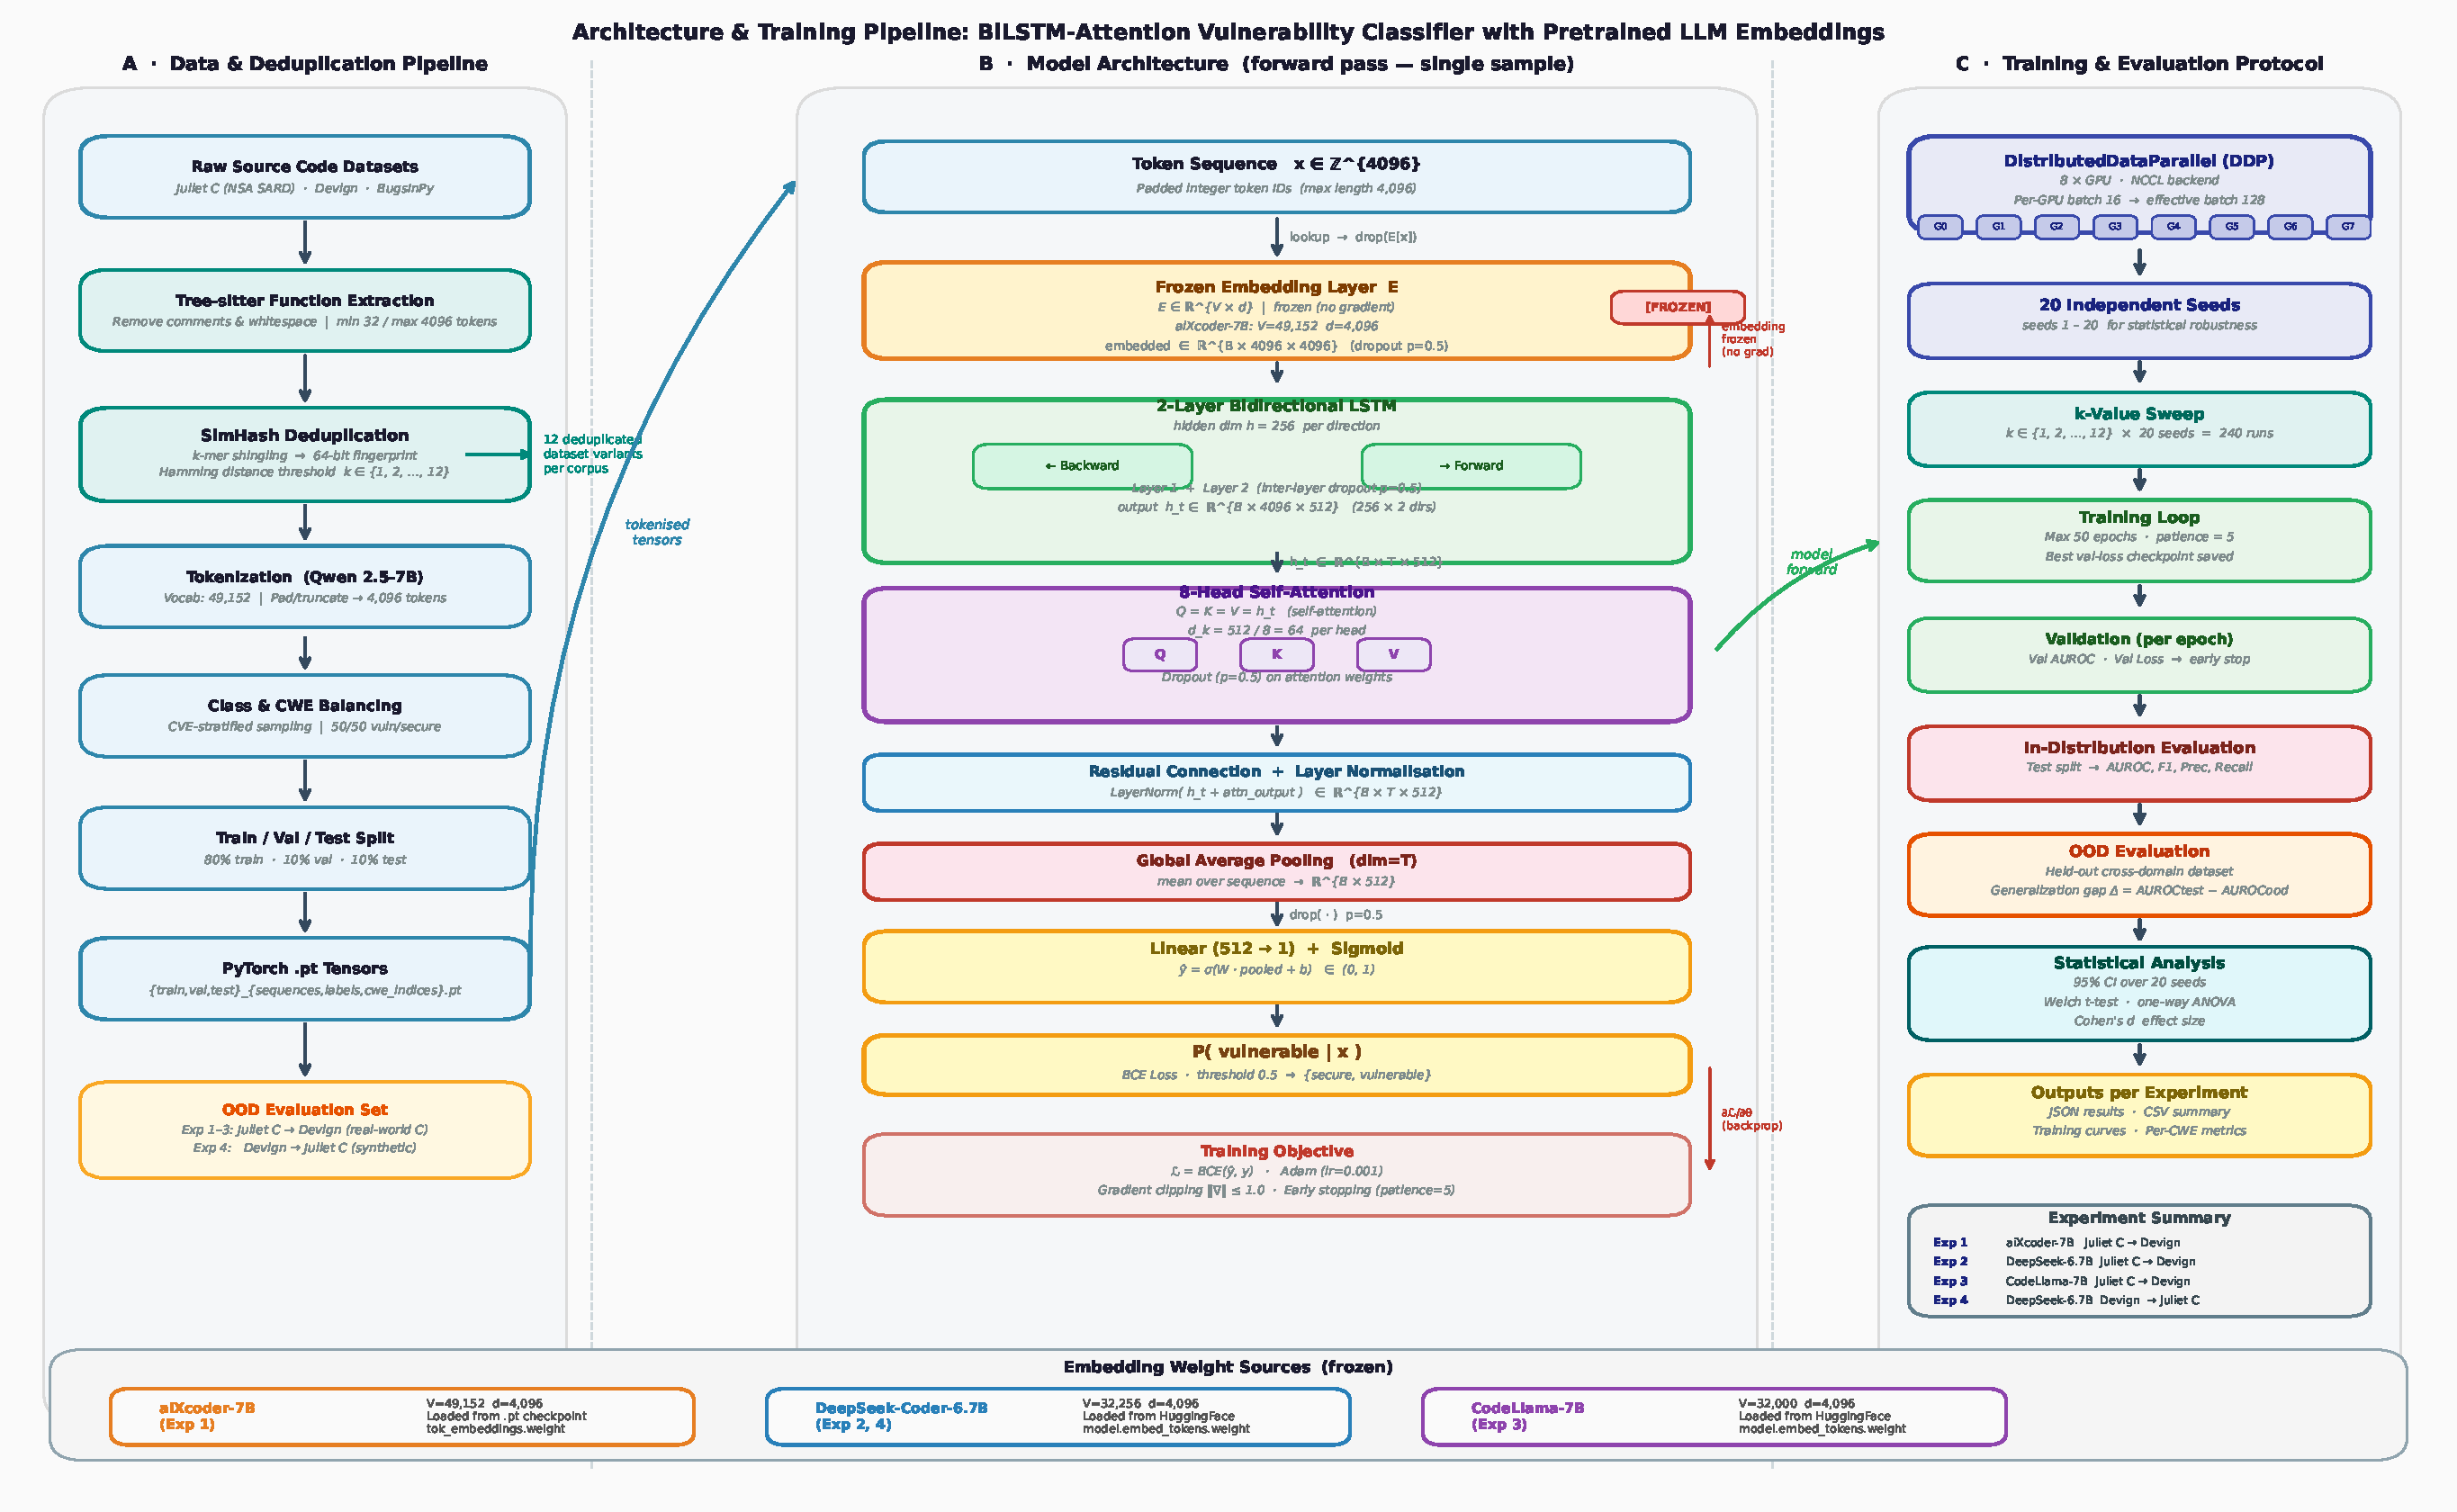
\includegraphics[width=\textwidth]{figures/model_architecture.pdf}
  \caption{%
    \textbf{Architecture and training pipeline.}
    \emph{(A) Data \& deduplication pipeline.}
    Raw source code is parsed into functions by Tree-sitter, tokenised with
    the Qwen~2.5-7B vocabulary (49{,}152 tokens), and deduplicated at twelve
    progressively stricter SimHash Hamming-distance thresholds
    ($k \in \{1,\dots,12\}$).
    Each threshold produces an independent dataset variant that is split into
    train / validation / test and serialised as PyTorch tensors.
    \emph{(B) Model forward pass.}
    A frozen embedding matrix $\mathbf{E} \in \mathbb{R}^{V \times d}$,
    sourced from a pretrained code LLM, projects each token sequence into a
    continuous representation.
    Two bidirectional LSTM layers with hidden dimension 256 produce
    contextualised token representations, which are refined by an
    8-head self-attention block with residual connection and layer
    normalisation.
    Global average pooling collapses the sequence dimension; a linear layer
    with sigmoid activation yields the final vulnerability probability.
    \emph{(C) Training \& evaluation protocol.}
    Each configuration is trained across 20~independent random seeds on
    8~GPUs via DistributedDataParallel.
    Final metrics are computed on a held-out in-distribution test split and a
    held-out out-of-distribution (OOD) dataset.%
  }
  \label{fig:architecture}
\end{figure*}

\subsection{Embedding Layer}
\label{sec:embedding}

The first layer of the classifier is an embedding table
$\mathbf{E} \in \mathbb{R}^{V \times d}$ whose weights are copied directly
from a pretrained code LLM and held \emph{frozen} (i.e., no gradients flow
through $\mathbf{E}$ during training).
This design choice is central to our experimental methodology: by preventing
the optimiser from modifying the embedding weights, any difference in
downstream task performance across experiments reflects purely the quality of
the pretrained representations, not the model's capacity to adapt them
through gradient descent.
The three embedding sources used across the four experiments are:

\begin{itemize}
  \item \textbf{aiXcoder-7B}~\cite{aixcoder}
        ($V = 49{,}152$, $d = 4{,}096$) — weights extracted from the
        \texttt{tok\_embeddings.weight} tensor of the local \texttt{.pt}
        checkpoint.  Used in Experiment~1.

  \item \textbf{DeepSeek-Coder-6.7B-Base}~\cite{deepseek}
        ($V = 32{,}256$, $d = 4{,}096$) — weights extracted from
        \texttt{model.embed\_tokens.weight} via HuggingFace \texttt{safetensors}.
        Used in Experiments~2 and~4.

  \item \textbf{CodeLlama-7B-hf}~\cite{rozière2024codellamaopenfoundation}
        ($V = 32{,}000$, $d = 4{,}096$) — weights extracted identically to
        DeepSeek-Coder.  Used in Experiment~3.
\end{itemize}

\noindent
In all cases the same Qwen~2.5-7B tokeniser (vocabulary size 49{,}152) is
used for tokenisation, creating a deliberate mismatch between the tokeniser
and the DeepSeek / CodeLlama embedding tables.
We retain this design as a controlled variable; the effect of model-specific
tokenisers is identified as future work (Section~\ref{sec:future_work}).

\subsection{Bidirectional LSTM}
\label{sec:lstm}

The embedded token sequence
$\mathbf{X} \in \mathbb{R}^{B \times T \times d}$ (batch size $B$, sequence
length $T \leq 4{,}096$, embedding dimension $d = 4{,}096$) is first passed
through a dropout layer ($p = 0.5$) before being fed into a two-layer
bidirectional LSTM.
Each LSTM layer maintains a hidden state of dimension $h = 256$ per
direction; the bidirectional configuration concatenates the forward
($\overrightarrow{\mathbf{h}}_t$) and backward
($\overleftarrow{\mathbf{h}}_t$) hidden states at each time step, yielding
an output tensor
$\mathbf{H} \in \mathbb{R}^{B \times T \times 2h}$ with $2h = 512$.
Inter-layer dropout ($p = 0.5$) is applied between the two LSTM layers.

The bidirectional architecture is chosen because vulnerability semantics
frequently require integrating leftward context (e.g., a variable
declaration) with rightward context (e.g., an unchecked pointer dereference
several lines later).
A unidirectional LSTM would process only the causal context, potentially
missing important backward dependencies.

\subsection{Multi-Head Self-Attention with Residual Connection}
\label{sec:attention}

The LSTM output $\mathbf{H}$ is passed to a multi-head self-attention
(MHSA) module~\cite{attention_is_all_you_need} with $N_h = 8$ heads and key
dimension $d_k = 2h / N_h = 64$ per head.
In the self-attention formulation, query, key, and value matrices are all
derived from $\mathbf{H}$:

\begin{equation}
  \text{MHSA}(\mathbf{H}) =
    \text{MultiHead}(\mathbf{H}\mathbf{W}_Q,\; \mathbf{H}\mathbf{W}_K,\;
                     \mathbf{H}\mathbf{W}_V),
  \label{eq:mhsa}
\end{equation}

\noindent where $\mathbf{W}_Q, \mathbf{W}_K, \mathbf{W}_V \in
\mathbb{R}^{512 \times 512}$ are learned projection matrices.
Dropout ($p = 0.5$) is applied to the attention weights before computing the
weighted values.

The self-attention output is combined with the original LSTM output via a
residual connection and normalised:

\begin{equation}
  \hat{\mathbf{H}} = \text{LayerNorm}\!\left(
    \mathbf{H} + \text{MHSA}(\mathbf{H})
  \right).
  \label{eq:residual}
\end{equation}

\noindent
This residual structure prevents degradation of the LSTM's sequential
features while allowing the attention mechanism to capture non-local
dependencies between distant tokens in the function body.
It mirrors the architectural pattern found in modern transformer encoder
blocks.

\subsection{Global Average Pooling and Classification Head}
\label{sec:head}

The attended sequence $\hat{\mathbf{H}} \in \mathbb{R}^{B \times T \times 512}$
is collapsed to a fixed-length vector by global average pooling over the
sequence dimension:

\begin{equation}
  \mathbf{p} = \frac{1}{T}\sum_{t=1}^{T} \hat{\mathbf{H}}_t
  \;\in\; \mathbb{R}^{B \times 512}.
  \label{eq:gap}
\end{equation}

\noindent
Global average pooling is preferred over taking the final hidden state of the
LSTM because it aggregates information from all positions uniformly,
providing a more stable gradient signal and making the classifier less
sensitive to the order in which vulnerability-related tokens appear in the
function.

A final dropout layer ($p = 0.5$) is applied before a linear classification
head maps the pooled representation to a scalar:

\begin{equation}
  \hat{y} = \sigma\!\left( \mathbf{W}_c \, \mathbf{p} + b_c \right),
  \label{eq:classifier}
\end{equation}

\noindent
where $\mathbf{W}_c \in \mathbb{R}^{1 \times 512}$, $b_c \in \mathbb{R}$,
and $\sigma$ denotes the logistic sigmoid.
The output $\hat{y} \in (0, 1)$ is interpreted as $P(\text{vulnerable} \mid
\mathbf{x})$; a threshold of $0.5$ is used for binary classification.

\subsection{Training Configuration}
\label{sec:training}

All models are trained with binary cross-entropy loss

\begin{equation}
  \mathcal{L} = -\left[
    y \log \hat{y} + (1 - y) \log (1 - \hat{y})
  \right],
  \label{eq:bce}
\end{equation}

\noindent
and optimised with Adam~\cite{adam} at a learning rate of $10^{-3}$.
Gradient norms are clipped at 1.0 to prevent exploding gradients in the
recurrent layers.
Training proceeds for a maximum of 50 epochs with early stopping based on
validation loss (patience = 5 epochs); the model checkpoint corresponding to
the lowest validation loss is restored before final evaluation.

Multi-GPU training is implemented with PyTorch
DistributedDataParallel~\cite{pytorch} over 8 GPUs using the NCCL backend.
The per-GPU batch size is 16, giving an effective batch size of 128.
Each experiment processes twelve deduplication levels
($k \in \{1, \dots, 12\}$) across 20 independent random seeds, yielding
$12 \times 20 = 240$ trained models per experiment and 960 models in total
across all four experiments.

Full hyperparameter details are summarised in Table~\ref{tab:model_config}.

\begin{table}[h]
\centering
\caption{Model architecture and training hyperparameters}
\label{tab:model_config}
\begin{tabular}{@{} l l @{}}
\toprule
\multicolumn{2}{c}{\textbf{Model Architecture}} \\
\midrule
\textbf{Component} & \textbf{Configuration} \\
\midrule
Embedding layer   & Vocab: $V$ tokens (see \S\ref{sec:embedding}); dim: 4{,}096; \textit{frozen} \\
LSTM layers       & 2 layers; hidden dim 256; bidirectional; inter-layer dropout 0.5 \\
Attention         & 8-head self-attention; $d_k = 64$; attention dropout 0.5 \\
Residual + norm   & LayerNorm after residual addition \\
Pooling           & Global average pooling over sequence dimension \\
Classification    & Linear (512 $\to$ 1) + sigmoid; pre-linear dropout 0.5 \\
\midrule
\multicolumn{2}{c}{\textbf{Training Hyperparameters}} \\
\midrule
Optimiser         & Adam \\
Learning rate     & $1 \times 10^{-3}$ \\
Loss function     & Binary cross-entropy \\
Effective batch   & 128 (16 per GPU $\times$ 8 GPUs) \\
Max epochs        & 50 \\
Early stopping    & Patience 5 (val loss) \\
Gradient clipping & $\|\nabla\|_2 \leq 1.0$ \\
Seeds per config  & 20 \\
Sequence length   & Min 32 / Max 4{,}096 tokens \\
\bottomrule
\end{tabular}
\end{table}

\subsection{Parameter Count and Complexity}
\label{sec:complexity}

The embedding layer dominates the parameter budget but is \emph{not trained},
contributing $V \times 4{,}096$ frozen parameters (approximately 200M for
aiXcoder, 132M for DeepSeek / CodeLlama).
The trainable parameters consist solely of the LSTM layers, attention
projections, layer normalisation, and classification head, totalling
approximately 37M parameters:

\begin{itemize}
  \item \textbf{LSTM} (2 layers, bidirectional, $d=4{,}096 \to h=256$):
        Layer 1 — $4 \times (4{,}096 + 256 + 1) \times 256 \times 2 \approx 8.8\text{M}$;
        Layer 2 — $4 \times (512 + 256 + 1) \times 256 \times 2 \approx 1.6\text{M}$.
  \item \textbf{Multi-head attention} (512-dim, 8 heads):
        $3 \times 512^2 + 512^2 = 4 \times 512^2 \approx 1.0\text{M}$.
  \item \textbf{Layer normalisation}: $2 \times 512 \approx 1{,}024$ parameters.
  \item \textbf{Classification head}: $512 + 1 = 513$ parameters.
\end{itemize}

\noindent
This compact trainable footprint (\textasciitilde12M parameters) allows each
seed to converge within minutes per epoch on 8 GPUs, making the 960-model
sweep computationally tractable at roughly 250 total GPU-hours.
It also ensures that any inter-experiment performance differences are not
confounded by differences in optimisable capacity.
